\section{Discoveries big and small in the Hollow mountain}

\begin{marginfigure}
\begin{tikzpicture}
\node [name-dest] (box){%
    \begin{minipage}{0.80\textwidth}
     \begin{itemize}
    \item Clare Tan
    \item Iztok Mozir
    \end{itemize}
    \end{minipage}

};
\node[fancytitle, right=10pt] at (box.north west) {Atlantis};
\end{tikzpicture}
\end{marginfigure}

\section{ At the end Atlantis}
Pushed Brezno Slapov with Izi last night, it was a great trip. Dropped a couple of pitches to get to a canyon/rift with a stream, followed it and eventually got to a sump. But taking a left turn down and inlet leads to the base of another wet pitch and a continuation of passage, but is was wet and we didn’t go on.
\name{Clare Tan}

\begin{marginfigure}
\centering
\frame{\includegraphics[width=\linewidth]{"images/2013/other-finds-2013/oli-fire".jpg}}
\label{Olifire}
\caption{On the last night on top of the mountain, all perishable food is ritually burned as Oliver Myerscough demonstrates with flour--- Kate Smith}
\end{marginfigure}

\section{Below Balamory}
\subsection{06/08/2013}
Exciting night of pushing yesterday. Clapton pitch is a massive space. Effectively like two shafts right next to each other. We drop the shorter one. Couple of leads at the bottom. One has abedding plane squeeze that stopped Maffi, it follows water to a small pitch, might join up with something off the other half of Clapton.
We mainly pushed the other lead, schematic on facing page. It’s still open and going. nfortunatley when we started to survey we discovered a crask in the clino glass. Which is why the tentative passage name is now CRACK SHACK [ed. not on page reads “Renamed PICK YOUR POSION]. There’s also alot of black sandy silt deposition in our passage, plus its in keepeing with the cocaine theme...
Going back today to survey waiting for day trainers to arrive, listening to music, writing this t put off pissing....I really like caving and camping underground...
P.S. none of the leads were killed during this push!!!!

\name{Clare Tan}

\subsection{07/08/2013}
Went back to Clapton yesterday to survey what we found the previous trip ~200m added to this years total. There are so many leads there we called it PICK YOUR POISON. Will be dreaming about it now for the next 11 months...
I guess this is now my last few hours in camp. It’s been a great expo of caving for me - many thanks to all my pushing/camping partners: Saber, Izi, Rhys and Maffi for the excellent trips and company. Thanks also to all who have camped at X-Ray for the laughs and great conversation.
Almost can;t believe another expo is drawing to a close...caving-wise I feel thoroughly satiated, but I’ve enjoyed myself so much that I don’t want it to end. Ah well, there’s always next year, and the year after, and the year after....I wonder if I’ll still be here in 10 years?
I should really go to sleep but my body doesn’t want to cooperate....Maybe it’s time to read Tet’s 15 page epic (from earlier in the expo.

\name{Clare Tan}

Still no inspiration, I guess Clare Tan has drained out of me even this, nor only all energy, while trying to figure out how to squeeze through thos passages we’ve found. Anyway it is the last day in X-Ray this year. Wish this refuge was open the whole year. Aja! I want to thank Dave Wilson for the hint on Balamory. He made possible the biggest discovery this year! And with this he also gave Erik and me the sensation of pioneers. Thanks Dave! (well this sensation we get every time we push something nice but this one could be compared with findings of Columbus, Marco Polo, Juri Gagarin :) ) Thank you Erik, thank you Clare Tan. Thank you everyone that made Mig adventures possible. Over an out.
\name{Grega Maffi}


\begin{figure*}[b!]
\begin{tikzpicture}
\node [name-dest] (box){%
    \begin{minipage}{0.95\textwidth}
    \begin{multicols}{2}
July 20$^{th}$ --- ‘Yesterday’s trip to Minestrone was a lot of fun. Looked at the little leads going off and Kate’s climb. All became little squeezes with no draught. Except a climb (cairn at base of it) around PSS 21 and PSS 24, which leads to a downward sloping body sized tube which draughts. I went down it a good 5-10m but it seems to go on forever and felt too commiting to do without help/rope. \emph{HASH} is a new lead found by Tim on the way back. Around 30-40m down Lost Miles from Hawaii is a climb up on the left hand side. PSS for Hash is at start of climb. Left at draughting body sized crawl as we were short of time.'
\name{Clare Tan}

July 22$^{nd}$ --- ‘Oh, also, we went and pushed \emph{HASH}, adding around 25 metres to what Tim et al had surveyed previously. Hash is fucking twatty and does continue beyond what we surveyed. Problem, only Tetley could fit through the squeezed just beyond our last survey leg. It was so close, just my shoulders are slightly too broad..with some tools we could’ve enlarged it but we would have had to gone back through to collect them. Beyond the squeeze, the passage continues upwards into a small chamber, 3m wide, 8m tall with a tight passage continuin off at the top. (all according to Tetley of course). Go push you narrow shouldered people.'
\name{Sam Page}

August 1$^{st}$ ---‘I am currently sat in a big silver bag in \emph{Friendship Gallery} with Clare. Today we pushed and killed \emph{Invictus}. It ends in a very tight rift with a puddle. The 20m of passage is named “\emph{RCC Passage of the Year}”. We also pushed \emph{Hash} to a tight chicane crawl thing that is is inadvisable for people bigger than Clare to go down. All in all got about 50m of passage. The silver bag, “Camp Gamma Ray” is very warm grim.'
\name{Rhys Tyers}
 \end{multicols}
    \end{minipage}

};
\node[fancytitle, right=10pt] at (box.north west) {The story of Hash};
\end{tikzpicture}
\end{figure*}

\begin{figure*}
      \checkoddpage \ifoddpage \forcerectofloat \else \forceversofloat \fi
      \centering
    \begin{subfigure}[t]{\textwidth}
    \centering
        \frame{\includegraphics[width=\linewidth]{"images/2013/other-finds-2013/lethe_sifon_2".jpg}} 
        \caption{} \label{Panorama}
    \end{subfigure}
    
          \vspace{0.3cm}
          
    \begin{subfigure}[t]{0.555\textwidth}
        \centering
        \frame{\includegraphics[width=\linewidth]{"images/2013/other-finds-2013/clare_in_lethe".jpg}} 
        \caption{} \label{Will Scott bolting}
    \end{subfigure}
    \hfill
    \begin{subfigure}[t]{0.418\textwidth}
        \centering
        \frame{\includegraphics[width=\linewidth]{"images/2013/other-finds-2013/lethe_canyon".jpg}} 
        \caption{} \label{Ice}
    \end{subfigure}

    \caption{
    \emph{a} The cascading steam from Brezno Slapov ends at an ominous sump (-802m)
    \emph{b} Clare Tan navigates through the stream and canyon passage below Brezno Slapov.
    \emph{c} Water from the stream passage accumulates in deep pools --- Iztok Mozir }
\end{figure*}

\begin{figure*}[h!]
      \checkoddpage \ifoddpage \forcerectofloat \else \forceversofloat \fi
      \centering
              \frame{\includegraphics[width=\linewidth]{"images/2013/other-finds-2013/kate-end-of-expo-2013".jpg}} 
       \label{Panorama}
  \caption{ --- Tim Child }
\end{figure*}




\begin{figure*}[t!]
\centering
\frame{\includegraphics[width=\textheight, angle=270]{"images/2013/other-finds-2013/2013plan".pdf}}
\caption{}
\label{}
\end{figure*}

\begin{figure*}[t!]
\centering
\frame{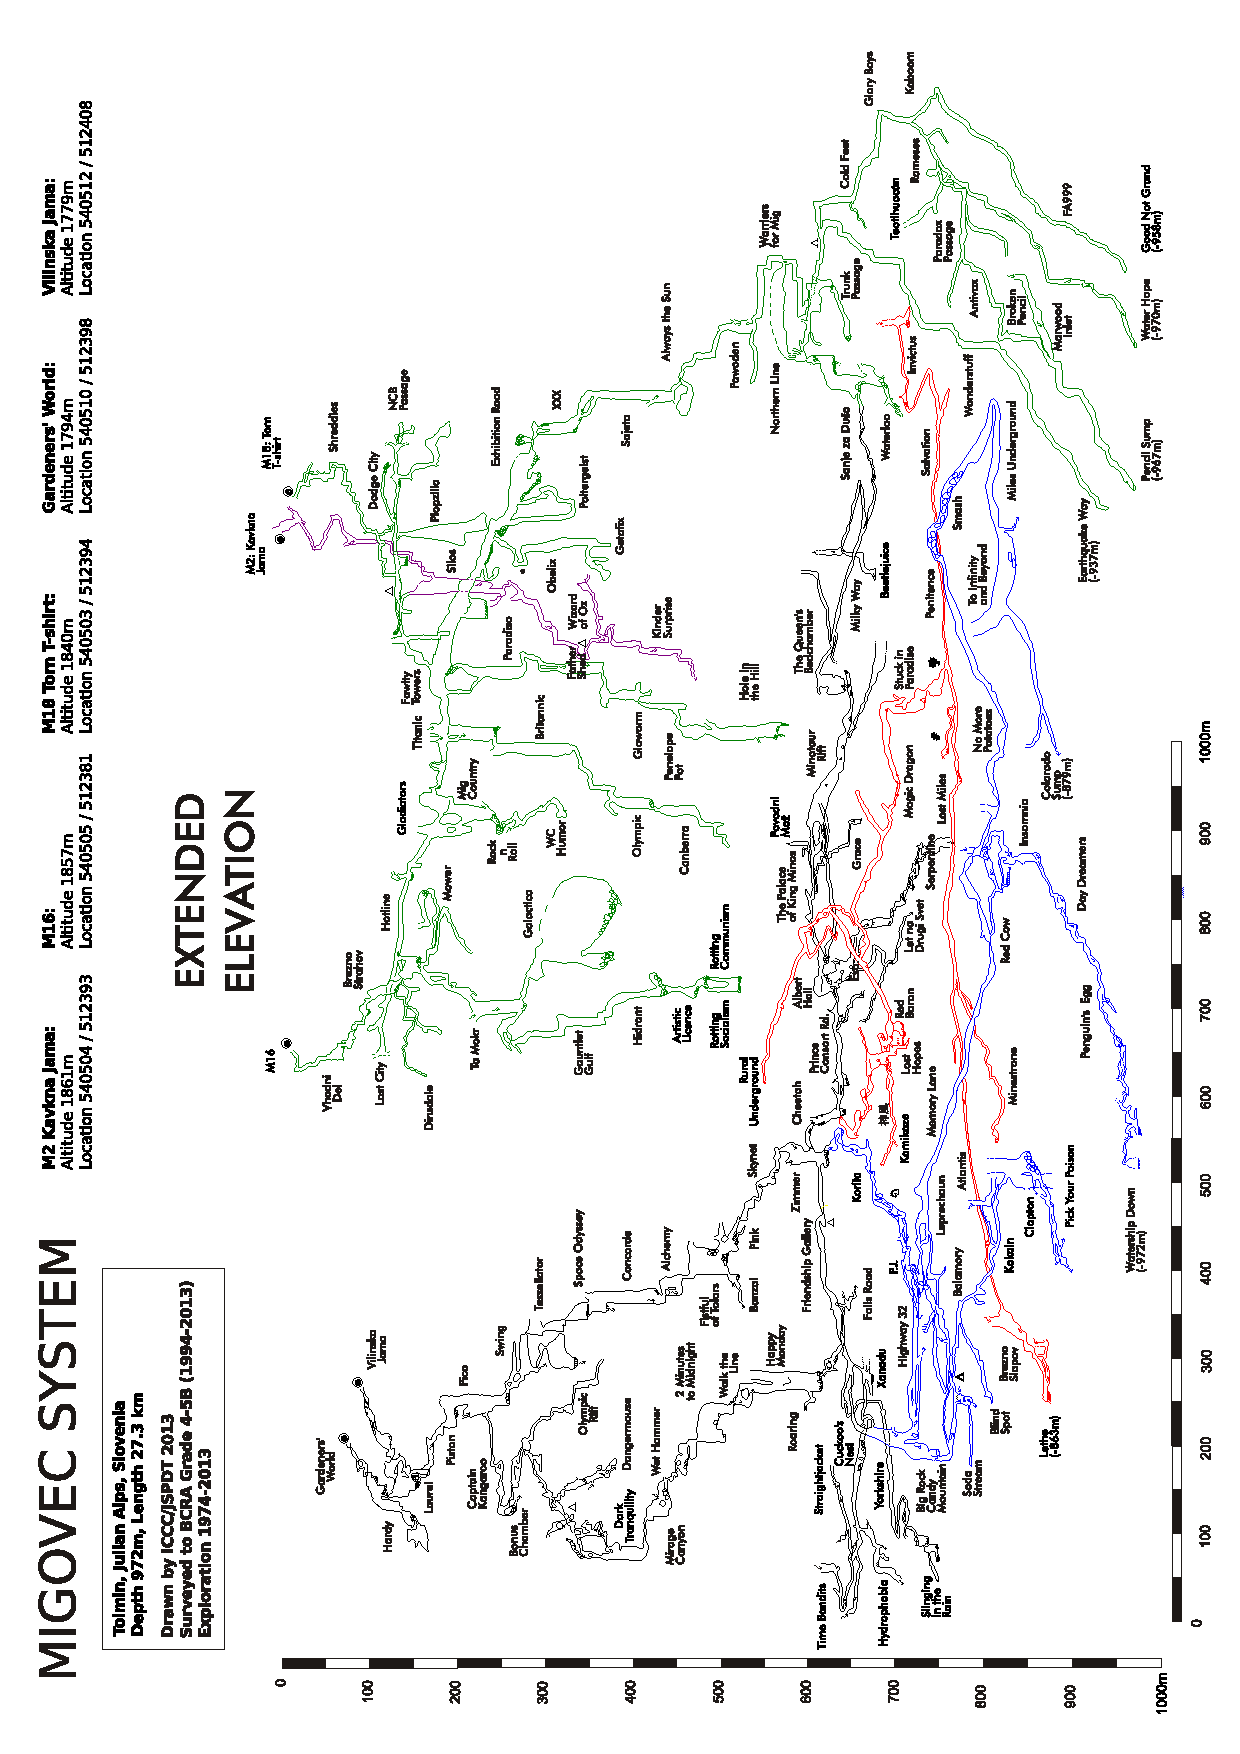
\includegraphics[height=\textheight]{images/2013/other-finds-2013/ee2013.pdf}}
\caption{}
\label{}
\end{figure*}